\chapter{Návrh a architektura aplikace}

\section{Serverová část}

Rozdělení do projektů:

TODO: u každé dopodrobna rozepsat co obsahuje, k čemu slouží + ukázky kódu

\subsection{Data}

Tento projekt se stará primárně o komunikaci s databází, pro tento účel jsem použil ORM framework Entity Framework Core. 

Ve složce Models jsou třídy reprezentující databázové entity. Každá z entit pak v databázi představuje jednu tabulku. V aplikaci jsem použil tyto entity:

\begin{itemize}
	\item Course - tato entita reprezentuje kurz
	\item CourseFile - reprezentuje nějaký soubor sdílený v kurzu
	\item CourseMember - představuje členství uživatele v daném kurzu. K této entitě se pak vážou všechny známky a odeslané testy.
	\item CourseTest - představuje jeden test v kurzu
	\item ForumPost - slouží k reprezentaci příspěvků ve fóru k danému kurzu
	\item Grade - reprezentuje známku kterou student obdržel (kromě známek z testů)
	\item Person - reprezentuje uživatele aplikace
	\item TestQuestion - reprezentuje 1 otázku v testu
	\item TestSubmission - reprezentuje test s odpověďmi odeslaný uživatelem
	\item TestSubmissionAnswer - představuje odpověď k dané otázce v testu
\end{itemize}

\newpage

\begin{figure}
	\centering
	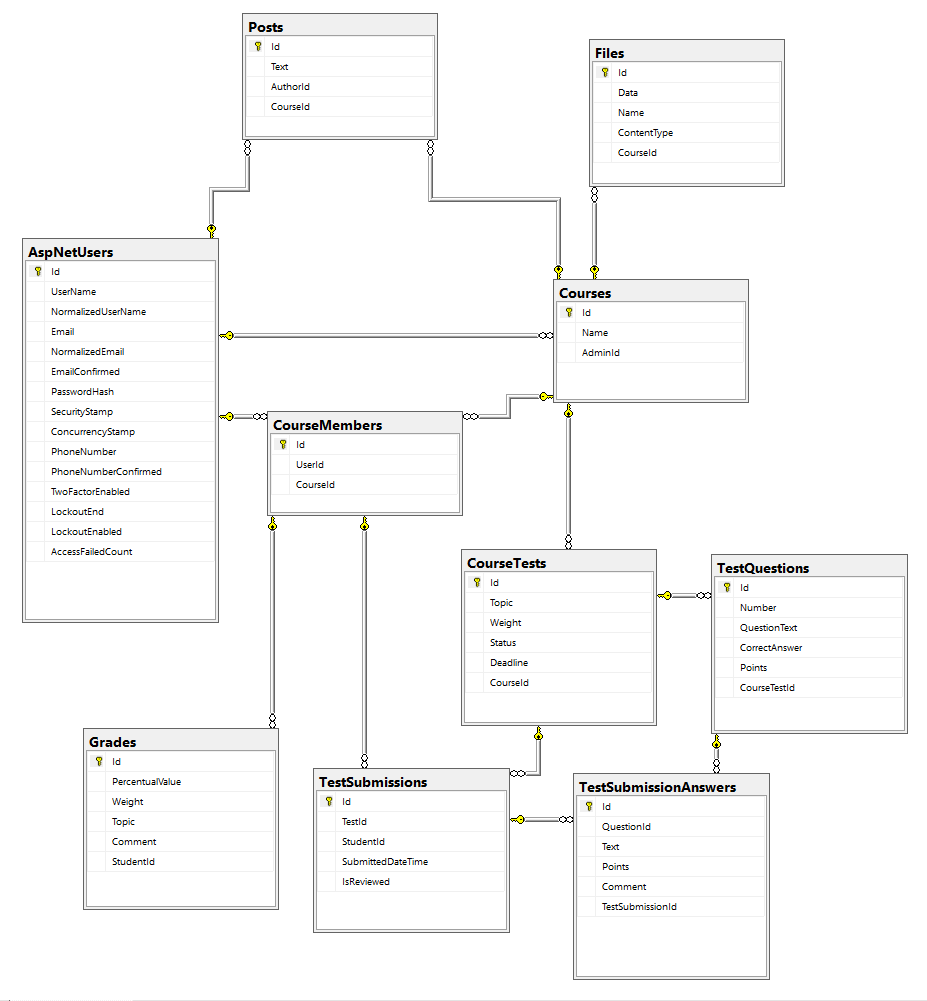
\includegraphics[width=\textwidth]{db_model.PNG}
	\caption{Databázový model aplikace}
\end{figure}

\newpage

např. kód třídy Course vypadá takto:

\begin{lstlisting}
public class Course : IGuidIdObject
{
	public Course()
	{
		Members = new List<CourseMember>();
		Files = new List<CourseFile>();
		Tests = new List<CourseTest>();
		ForumPosts = new List<ForumPost>();
	}
	
	public Course(string name, Person admin) : this()
	{
		Name = name;
		Admin = admin;
	}
	
	/// <summary>
	/// identifier of the couse
	/// </summary>
	[DatabaseGenerated(DatabaseGeneratedOption.Identity)]
	[Key]
	public Guid Id { get; set; }
	
	/// <summary>
	/// name of the course
	/// </summary>
	[Required]
	public string Name { get; set; }
	
	/// <summary>
	/// admin of the course
	/// </summary>
	[Required]
	public Person Admin { get; set; }
	
	/// <summary>
	/// members of the course (except admin)
	/// </summary>
	public ICollection<CourseMember> Members { get; set; }
	
	/// <summary>
	/// shared files in this course
	/// </summary>
	public ICollection<CourseFile> Files { get; set; }
	
	/// <summary>
	/// tests in this course
	/// </summary>
	public ICollection<CourseTest> Tests { get; set; }
	
	/// <summary>
	/// posts in the forum of this course
	/// </summary>
	public ICollection<ForumPost> ForumPosts { get; set; }
}
\end{lstlisting}

Vidíme, že každá entita obsahuje veřejné vlastnosti (public properties) s gettery a settery. Tyto vlastnosti budou v databázové tabulce reprezentovány jako sloupce. Některé vlastnosti (jako např. Id) obsahují ještě doplňující atributy, ty slouží k upřesnění informací o dané vlastnosti. Například atribut [Key] určuje, že tato vlastnost bude v databázi primární klíč, atribut [Required] určuje, že daný sloupec bude v tabulce u všech záznamů povinný (tedy hodnoty budou NOT NULL).
Dále musí každá entita obsahovat konstruktor bez parametrů.

Vazby mezi entitami jsou reprezentované pomocí tzv. navigačních vlastností. V případě, že chci vytvořit vazbu typu one-to-many mezi entitami A a B, tak stačí do vlastností třídy A přidat kolekci objektů typu B, a naopak do třídy B vlastnost typu A. Framework pak při provádění migrace vytvoří v databázové tabulce entity B vytvoří sloupec s cizím klíčem, který bude obsahovat identifikátor entity A, ke které patří.

V aplikaci je vazba one-to-many použita mimo jiné mezi entitami Course a CourseTest, a to tak, že každý test je obsažen v právě jednom kurzu, a v daném kurzu může být N testů.
Kód pak tedy vypadá takto: ve třídě Course je kolekce objektů typu CourseTest

\begin{lstlisting}
/// <summary>
/// tests in this course
/// </summary>
public ICollection<CourseTest> Tests { get; set; }
\end{lstlisting}

a ve třídě CourseTest je pak vlastnost typu Course

\begin{lstlisting}
/// <summary>
/// course that contains this test
/// </summary>
[Required]
public Course Course { get; set; }
\end{lstlisting}

Po provedení databázové migrace (viz. dále) se v tabulce CourseTest vytvoří sloupec CourseId s cizím klíčem, který odkazuje na identifikátor kurzu (tzn. vlastnost Course.Id).

Také si můžeme všimnout, že všechny entity (kromě entity Person) implementují rozhraní IGuidObject. To je jednoduché rozhraní, které obsahuje pouze jednu vlastnost - Id typu Guid. Tímto jsem si zajistil jednotu identifikátorů, tedy že všechny entity, které toto rozhraní implementují, budou mít identifikátor typu Guid.

\begin{lstlisting}
/// <summary>
/// interface for object with <see cref="Guid"/> identifier
/// </summary>
public interface IGuidIdObject
{
	/// <summary>
	/// identifier of the object
	/// </summary>
	Guid Id { get; set; }
}
\end{lstlisting}


Pro typ Guid jsem se rozhodl hlavně z toho důvodu, že vestavěné tabulky frameworku (např. Identity) mají také řetězcové identifikátory. Navíc se pak zjednoduší práce ve frontend části (není potřeba parsovat string na int např. v klientské části při práci s URL). Tyto identifikátory generuje databáze, takže je zajištěno, že jsou unikátní.
Další možnost by byla použít jako identifikátor číslo (např. typ int), ale vzhledem k výše uvedeným argumentům je typ Guid v tomto případě lepší možnost.

Dále jsou v projektu také rozhraní ICourseReferenceObject a ICourseMemberReferenceObject, které slouží k tomu, abychom mohli dále v aplikaci jednotně pracovat s objekty, které mají referenci na entitu Course, resp. CourseMember. Tyto rozhraní implementují pouze nějaké entity.

V programu je dále třída CMSDbContext, která reprezentuje databázový kontext této aplikace. Každý objekt typu DbSet pak představuje jednu databázovou tabulku. Ve třídě je CMSDbContext tedy kolekce typu DbSet pro každou z entit.

\begin{lstlisting}
public DbSet<Grade> Grades { get; set; }

public DbSet<Course> Courses { get; set; }

public DbSet<CourseMember> CourseMembers { get; set; }

public DbSet<CourseFile> Files { get; set; }

public DbSet<CourseTest> CourseTests { get; set; }

public DbSet<TestQuestion> TestQuestions { get; set; }

public DbSet<TestSubmission> TestSubmissions { get; set; }

public DbSet<TestSubmissionAnswer> TestSubmissionAnswers { get; set; }

public DbSet<ForumPost> Posts { get; set; }
\end{lstlisting}

Jediná výjimka je entita Person, která dědí z třídy IdentityUser, a jejíž DbSet je nakonfigurovaný ve frameworku. 

V programu pak dále používám ke komunikaci s databází pouze třídu CMSDbContext a objekty typu DbSet. Třida DbSet<TEntity> implementuje rozhraní IQueryable<TEntity>, takže na ní lze použít LINQ. Takže pokud bych chtěl například vybrat všechny kurzy, jejiž jméno začíná na písmeno C, tak stačí použít LINQ dotaz
\begin{lstlisting}
dbContext.Courses.Where(course => course.Name.StartsWith("C"))
\end{lstlisting}
kde proměnná dbContext je instance třídy CMSDbContext.

V programu je dále složka Migrations. Při vývoji jsem používal princip Code first, tedy že v kódu specifikuji entity pomocí klasických tříd. Framework se pak postará o vytvoření databázových tabulek z tohoto kódu.

Pokud jsem tedy nějak změnil některou z entit (to může být např. přidání vlastnosti, změna jména vlastnosti, apod.), tak pomocí ORM mohu vygenerovat soubor popisující tzv. databázovou migraci, která slouží k aplikaci změn z kódu do databáze. Ke každé migraci se vygeneruje jeden soubor, který obsahuje popis změn, které se později provedou v databázi.

K vytváření migrací jsem použil nástroj CLI tools for Entity Framework Core. https://docs.microsoft.com/cs-cz/ef/core/cli/dotnet. Pro vygenerování migrace ze změn v kódu jsem potom použil příkaz:

\begin{lstlisting}
dotnet ef migrations add {migration_name} 
--project CourseManagementSystem.Data 
--startup-project CourseManagementSystem.API
\end{lstlisting}

Tímto se vytvoří soubor popisující změny v migraci, ale databáze zatím zůstala beze změny. Tento soubor obsahuje třídu, jenž dědí ze třídy Migration a obsahuje metody Up a Down. V metodě Up je popis změn, které se provedou při aplikaci této migrace, naopak v metodě Down je popis změn, které se provedou v případě odstranění migrace.

Jako příklad jsem si vybral migraci, která obsahuje přidání vlastnosti ScoreWeight k entitě CourseTest (tato vlastnost popisuje váhu testu).
Vygenerovaný kód migrace pak vypadá takto:

\begin{lstlisting}
public partial class TestWeight_added : Migration
{
	protected override void Up(MigrationBuilder migrationBuilder)
	{
		migrationBuilder.AddColumn<int>(
		name: "ScoreWeight",
		table: "CourseTests",
		nullable: false,
		defaultValue: 0);
	}
	
	protected override void Down(MigrationBuilder migrationBuilder)
	{
		migrationBuilder.DropColumn(
		name: "ScoreWeight",
		table: "CourseTests");
	}
}
\end{lstlisting}

Pro promítnutí změn do databáze jsem pak použil příkaz:

\begin{lstlisting}
dotnet ef database update 
--project CourseManagementSystem.Data 
--startup-project CourseManagementSystem.API
\end{lstlisting}

Tímto tedy dojde k změnám v databázi (v našem příkladu se vytvoří sloupec ScoreWeight v tabulce CourseTests).

V obou příkazech je potřeba specifikovat cílový a startup projekt. Cílový projekt je ten, který obsahuje databázový kontext a entity naší aplikace (v tomto případě projekt Data). Naopak startup projekt je projekt, který je spouštěný frameworkem, což je potřeba pro získání konfiguračních informací o projektu, jako je například connection string do naší databáze.

\newpage

\subsection{Services}

obsahuje pomocné služby pro komunikaci s databází, 

\subsection{API}

obsahuje Controllery, ViewModels, komunikace s klientskou částí

\subsection{Tests}

obsahuje testy služeb

\section{Klientská část}

\subsection{Components}

slouží k zobrazování dat, každá komponenta má 2 části: šablonu a backend

\subsection{Services}

slouží ke komunikaci klienta se server části

\subsection{ViewModels}

reprezentují objekty, které se používají v komunikaci s API

\section{Zajímavé problémy}

\subsection{Použití Dependency injection}

TODO: popsat použití + ukázat příklad

\subsection{ViewModels x DB entity}

Použil jsem různé objekty pro databázové entity a view-modely.

TODO: pořádně rozepsat + vysvětlit + ukázka kódu

\subsection{ViewModels v serverové i klientské části}

view-modely jsou v serverové i klientské části aplikace

TODO: pořádně rozepsat + vysvětlit + ukázka kódu

\subsection{Uživatelské role}

V systému je několik rolí, serverová část provádí autorizaci.

TODO: pořádně rozepsat typy rolí + autorizaci
